\documentclass{standalone}
\usepackage{tikz}
\usetikzlibrary{patterns, positioning}
\usepackage[sfdefault]{ClearSans} %% option 'sfdefault' activates Clear Sans as the default text font
\usepackage[T1]{fontenc}

\begin{document}
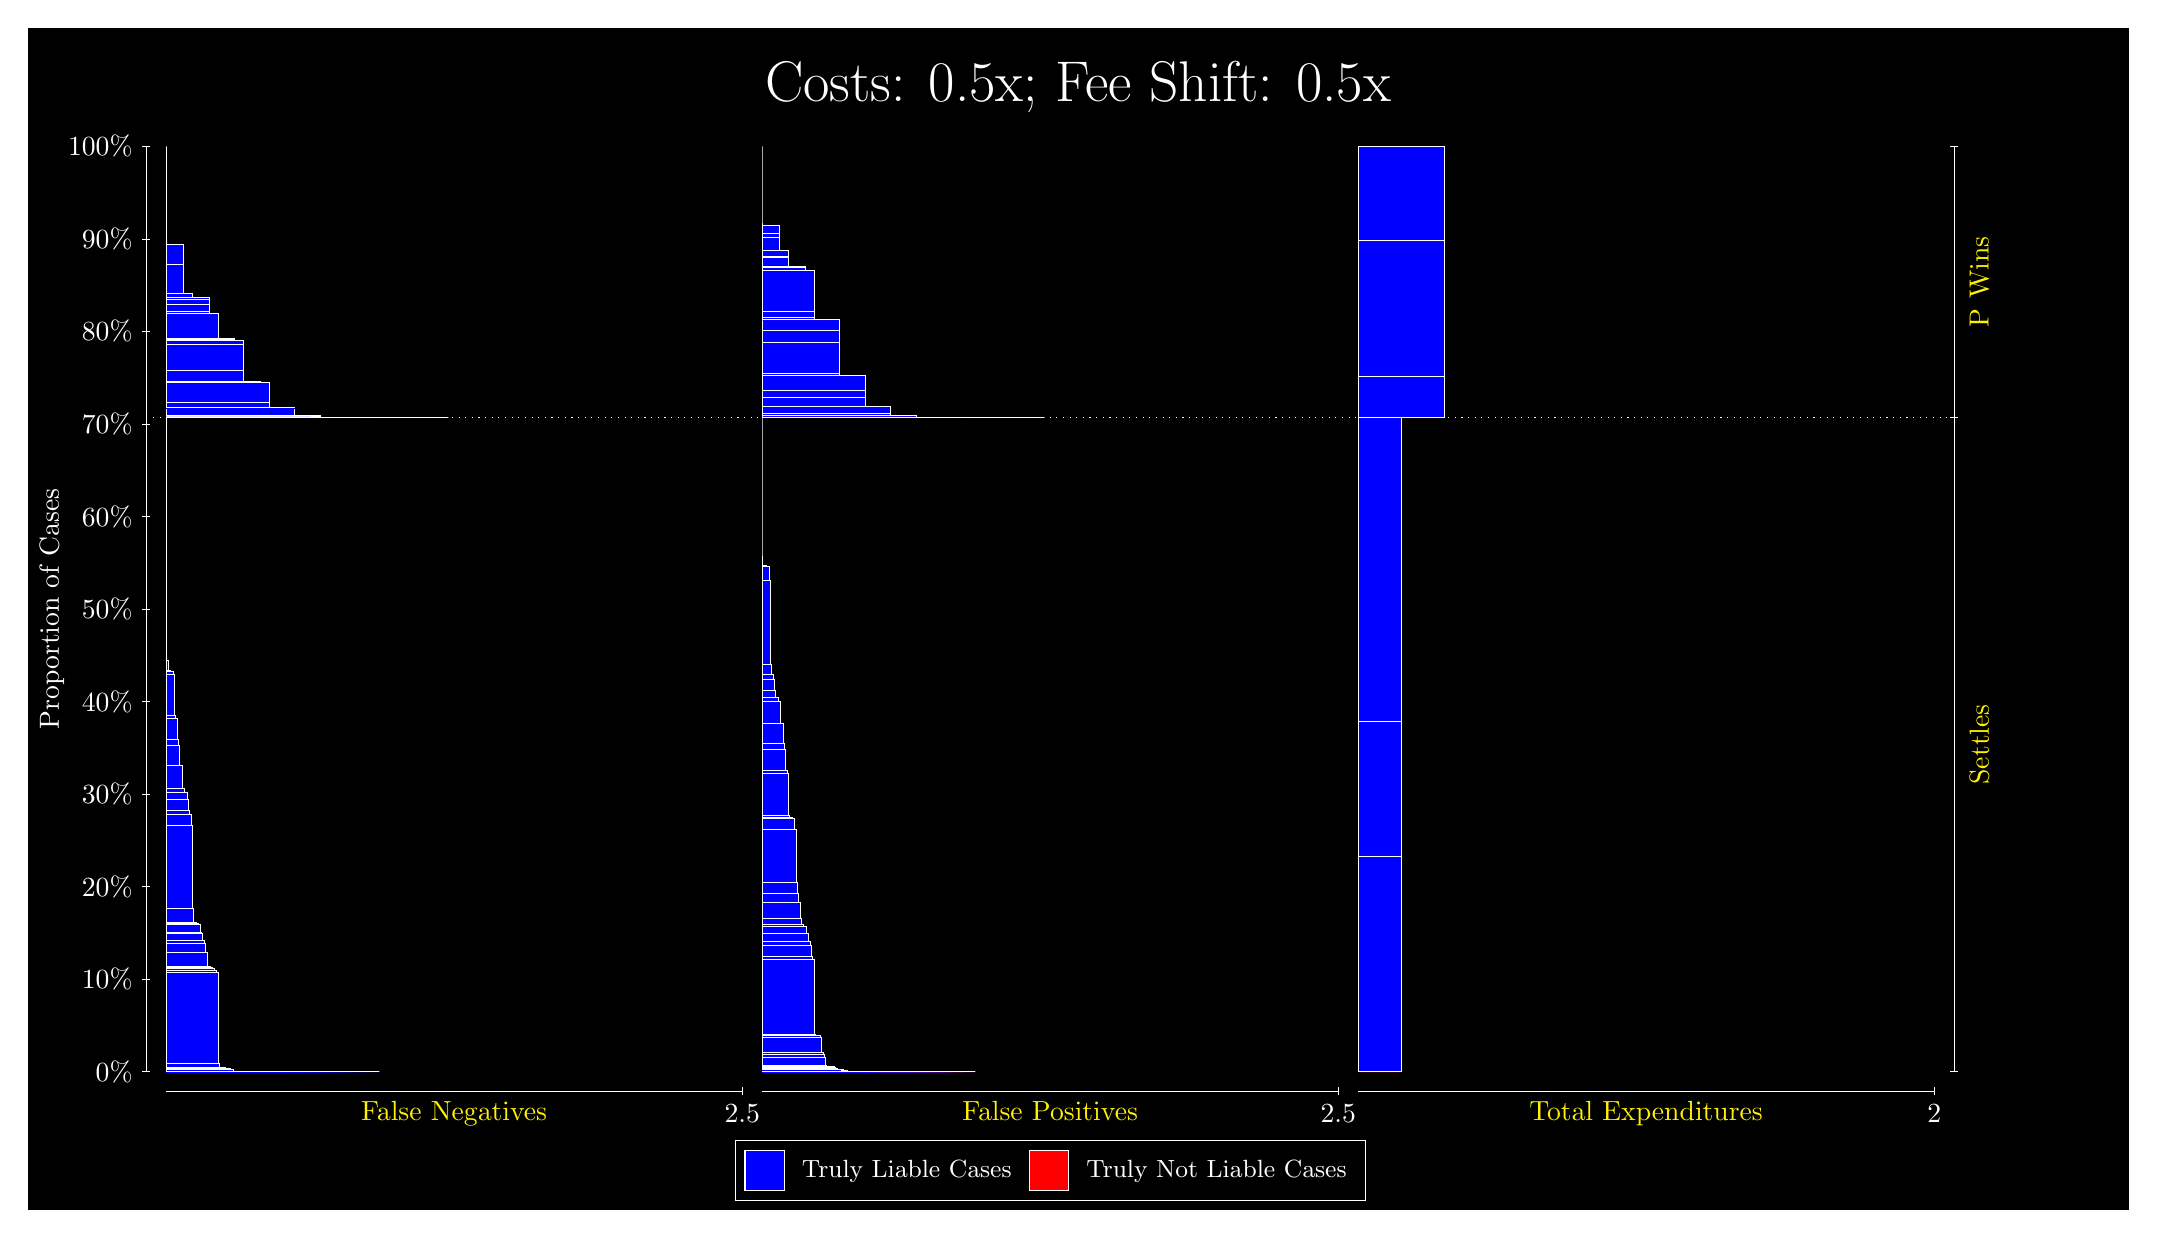
\begin{tikzpicture}
\draw[fill=black] (0,0) rectangle (26.667,15);
\draw[text=white] (0,13.5) rectangle (26.667,15) node[midway] {\huge Costs: 0.5x; Fee Shift: 0.5x};
\draw[white, very thin] (1.5,1.75) -- (1.5,13.5);
\node[rotate=90, text=white, anchor=center] at (0.3, 7.625) {Proportion of Cases};
\draw[white, very thin] (1.45,1.75) -- (1.55,1.75);
\node[text=white, anchor=east] at (1.45, 1.75) {0\%};
\draw[white, very thin] (1.45,2.925) -- (1.55,2.925);
\node[text=white, anchor=east] at (1.45, 2.925) {10\%};
\draw[white, very thin] (1.45,4.1) -- (1.55,4.1);
\node[text=white, anchor=east] at (1.45, 4.1) {20\%};
\draw[white, very thin] (1.45,5.275) -- (1.55,5.275);
\node[text=white, anchor=east] at (1.45, 5.275) {30\%};
\draw[white, very thin] (1.45,6.45) -- (1.55,6.45);
\node[text=white, anchor=east] at (1.45, 6.45) {40\%};
\draw[white, very thin] (1.45,7.625) -- (1.55,7.625);
\node[text=white, anchor=east] at (1.45, 7.625) {50\%};
\draw[white, very thin] (1.45,8.8) -- (1.55,8.8);
\node[text=white, anchor=east] at (1.45, 8.8) {60\%};
\draw[white, very thin] (1.45,9.975) -- (1.55,9.975);
\node[text=white, anchor=east] at (1.45, 9.975) {70\%};
\draw[white, very thin] (1.45,11.15) -- (1.55,11.15);
\node[text=white, anchor=east] at (1.45, 11.15) {80\%};
\draw[white, very thin] (1.45,12.325) -- (1.55,12.325);
\node[text=white, anchor=east] at (1.45, 12.325) {90\%};
\draw[white, very thin] (1.45,13.5) -- (1.55,13.5);
\node[text=white, anchor=east] at (1.45, 13.5) {100\%};

\draw[white, very thin] (24.457,1.75) -- (24.457,13.5);
\draw[white, very thin] (24.407,1.75) -- (24.507,1.75);
\node[anchor=west] at (24.407, 1.75) {};
\draw[white, very thin] (24.407,10.06) -- (24.507,10.06);
\node[anchor=west] at (24.407, 10.06) {};
\draw[white, very thin] (24.407,13.5) -- (24.507,13.5);
\node[anchor=west] at (24.407, 13.5) {};

\draw[white, very thin, fill=blue] (1.75,1.75) rectangle (4.458,1.75);
\draw[white, very thin, fill=blue] (1.75,1.75) rectangle (4.3116,1.75);
\draw[white, very thin, fill=blue] (1.75,1.75) rectangle (4.1652,1.75);
\draw[white, very thin, fill=blue] (1.75,1.75) rectangle (4.1327,1.75);
\draw[white, very thin, fill=blue] (1.75,1.75) rectangle (4.0188,1.75);
\draw[white, very thin, fill=blue] (1.75,1.75) rectangle (3.9863,1.75);
\draw[white, very thin, fill=blue] (1.75,1.75) rectangle (3.8725,1.75);
\draw[white, very thin, fill=blue] (1.75,1.75) rectangle (3.8399,1.75);
\draw[white, very thin, fill=blue] (1.75,1.75) rectangle (3.8074,1.75);
\draw[white, very thin, fill=blue] (1.75,1.75) rectangle (3.7261,1.75);
\draw[white, very thin, fill=blue] (1.75,1.75) rectangle (3.6936,1.75);
\draw[white, very thin, fill=blue] (1.75,1.75) rectangle (3.661,1.75);
\draw[white, very thin, fill=blue] (1.75,1.75) rectangle (3.5797,1.75);
\draw[white, very thin, fill=blue] (1.75,1.75) rectangle (3.5472,1.75);
\draw[white, very thin, fill=blue] (1.75,1.75) rectangle (3.5147,1.75);
\draw[white, very thin, fill=blue] (1.75,1.75) rectangle (3.4821,1.75);
\draw[white, very thin, fill=blue] (1.75,1.75) rectangle (3.4333,1.75);
\draw[white, very thin, fill=blue] (1.75,1.75) rectangle (3.4008,1.75);
\draw[white, very thin, fill=blue] (1.75,1.75) rectangle (3.3683,1.75);
\draw[white, very thin, fill=blue] (1.75,1.75) rectangle (3.3358,1.75);
\draw[white, very thin, fill=blue] (1.75,1.75) rectangle (3.287,1.75);
\draw[white, very thin, fill=blue] (1.75,1.75) rectangle (3.2544,1.75);
\draw[white, very thin, fill=blue] (1.75,1.75) rectangle (3.2219,1.75);
\draw[white, very thin, fill=blue] (1.75,1.75) rectangle (3.1894,1.75);
\draw[white, very thin, fill=blue] (1.75,1.75) rectangle (3.1568,1.75);
\draw[white, very thin, fill=blue] (1.75,1.75) rectangle (3.1406,1.75);
\draw[white, very thin, fill=blue] (1.75,1.75) rectangle (3.1081,1.75);
\draw[white, very thin, fill=blue] (1.75,1.75) rectangle (3.0755,1.75);
\draw[white, very thin, fill=blue] (1.75,1.75) rectangle (3.043,1.75);
\draw[white, very thin, fill=blue] (1.75,1.75) rectangle (3.0105,1.75);
\draw[white, very thin, fill=blue] (1.75,1.75) rectangle (2.9942,1.75);
\draw[white, very thin, fill=blue] (1.75,1.75) rectangle (2.9617,1.75);
\draw[white, very thin, fill=blue] (1.75,1.75) rectangle (2.9292,1.7505);
\draw[white, very thin, fill=blue] (1.75,1.7505) rectangle (2.8966,1.7506);
\draw[white, very thin, fill=blue] (1.75,1.7506) rectangle (2.8641,1.7507);
\draw[white, very thin, fill=blue] (1.75,1.7507) rectangle (2.8478,1.7507);
\draw[white, very thin, fill=blue] (1.75,1.7507) rectangle (2.8316,1.7507);
\draw[white, very thin, fill=blue] (1.75,1.7507) rectangle (2.8153,1.7508);
\draw[white, very thin, fill=blue] (1.75,1.7508) rectangle (2.7828,1.7508);
\draw[white, very thin, fill=blue] (1.75,1.7508) rectangle (2.7502,1.7529);
\draw[white, very thin, fill=blue] (1.75,1.7529) rectangle (2.7177,1.7535);
\draw[white, very thin, fill=blue] (1.75,1.7535) rectangle (2.7015,1.7539);
\draw[white, very thin, fill=blue] (1.75,1.7539) rectangle (2.6852,1.7544);
\draw[white, very thin, fill=blue] (1.75,1.7544) rectangle (2.6689,1.7549);
\draw[white, very thin, fill=blue] (1.75,1.7549) rectangle (2.6364,1.756);
\draw[white, very thin, fill=blue] (1.75,1.756) rectangle (2.6039,1.7776);
\draw[white, very thin, fill=blue] (1.75,1.7776) rectangle (2.5713,1.7863);
\draw[white, very thin, fill=blue] (1.75,1.7863) rectangle (2.5551,1.7903);
\draw[white, very thin, fill=blue] (1.75,1.7903) rectangle (2.5388,1.7963);
\draw[white, very thin, fill=blue] (1.75,1.7963) rectangle (2.5225,1.7965);
\draw[white, very thin, fill=blue] (1.75,1.7965) rectangle (2.5063,1.8017);
\draw[white, very thin, fill=blue] (1.75,1.8017) rectangle (2.49,1.8026);
\draw[white, very thin, fill=blue] (1.75,1.8026) rectangle (2.4575,1.8043);
\draw[white, very thin, fill=blue] (1.75,1.8043) rectangle (2.425,1.8488);
\draw[white, very thin, fill=blue] (1.75,1.8488) rectangle (2.4087,3.009);
\draw[white, very thin, fill=blue] (1.75,3.009) rectangle (2.3924,3.0307);
\draw[white, very thin, fill=blue] (1.75,3.0307) rectangle (2.3762,3.0384);
\draw[white, very thin, fill=blue] (1.75,3.0384) rectangle (2.3599,3.0574);
\draw[white, very thin, fill=blue] (1.75,3.0574) rectangle (2.3436,3.0732);
\draw[white, very thin, fill=blue] (1.75,3.0732) rectangle (2.3111,3.0914);
\draw[white, very thin, fill=blue] (1.75,3.0914) rectangle (2.2786,3.2699);
\draw[white, very thin, fill=blue] (1.75,3.2699) rectangle (2.2461,3.3831);
\draw[white, very thin, fill=blue] (1.75,3.3831) rectangle (2.2298,3.4106);
\draw[white, very thin, fill=blue] (1.75,3.4106) rectangle (2.2135,3.5093);
\draw[white, very thin, fill=blue] (1.75,3.5093) rectangle (2.1973,3.5158);
\draw[white, very thin, fill=blue] (1.75,3.5158) rectangle (2.181,3.6245);
\draw[white, very thin, fill=blue] (1.75,3.6245) rectangle (2.1647,3.6368);
\draw[white, very thin, fill=blue] (1.75,3.6368) rectangle (2.1322,3.6483);
\draw[white, very thin, fill=blue] (1.75,3.6483) rectangle (2.0997,3.826);
\draw[white, very thin, fill=blue] (1.75,3.826) rectangle (2.0834,4.8821);
\draw[white, very thin, fill=blue] (1.75,4.8821) rectangle (2.0672,5.0145);
\draw[white, very thin, fill=blue] (1.75,5.0145) rectangle (2.0509,5.074);
\draw[white, very thin, fill=blue] (1.75,5.074) rectangle (2.0346,5.2117);
\draw[white, very thin, fill=blue] (1.75,5.2117) rectangle (2.0184,5.3021);
\draw[white, very thin, fill=blue] (1.75,5.3021) rectangle (1.9858,5.3521);
\draw[white, very thin, fill=blue] (1.75,5.3521) rectangle (1.9533,5.636);
\draw[white, very thin, fill=blue] (1.75,5.636) rectangle (1.9208,5.8943);
\draw[white, very thin, fill=blue] (1.75,5.8943) rectangle (1.9045,5.971);
\draw[white, very thin, fill=blue] (1.75,5.971) rectangle (1.8882,6.2324);
\draw[white, very thin, fill=blue] (1.75,6.2324) rectangle (1.872,6.2728);
\draw[white, very thin, fill=blue] (1.75,6.2728) rectangle (1.8557,6.7993);
\draw[white, very thin, fill=blue] (1.75,6.7993) rectangle (1.8395,6.8296);
\draw[white, very thin, fill=blue] (1.75,6.8296) rectangle (1.8069,6.842);
\draw[white, very thin, fill=blue] (1.75,6.842) rectangle (1.7744,6.9784);
\draw[white, very thin, fill=blue] (1.75,6.9784) rectangle (1.7581,7.6575);
\draw[white, very thin, fill=red] (1.75,7.6575) rectangle (1.75,7.6575);
\draw[white, very thin, fill=blue] (1.75,7.6575) rectangle (1.75,10.06);
\draw[white, very thin, fill=blue] (1.75,10.06) rectangle (5.3362,10.06);
\draw[white, very thin, fill=blue] (1.75,10.06) rectangle (5.011,10.06);
\draw[white, very thin, fill=blue] (1.75,10.06) rectangle (4.6857,10.06);
\draw[white, very thin, fill=blue] (1.75,10.06) rectangle (4.3604,10.06);
\draw[white, very thin, fill=blue] (1.75,10.06) rectangle (4.2465,10.06);
\draw[white, very thin, fill=blue] (1.75,10.06) rectangle (4.0351,10.061);
\draw[white, very thin, fill=blue] (1.75,10.061) rectangle (4.0351,10.062);
\draw[white, very thin, fill=blue] (1.75,10.062) rectangle (3.9213,10.062);
\draw[white, very thin, fill=blue] (1.75,10.062) rectangle (3.7098,10.071);
\draw[white, very thin, fill=blue] (1.75,10.071) rectangle (3.7098,10.081);
\draw[white, very thin, fill=blue] (1.75,10.081) rectangle (3.596,10.081);
\draw[white, very thin, fill=blue] (1.75,10.081) rectangle (3.3845,10.18);
\draw[white, very thin, fill=blue] (1.75,10.18) rectangle (3.3845,10.183);
\draw[white, very thin, fill=blue] (1.75,10.183) rectangle (3.2707,10.183);
\draw[white, very thin, fill=blue] (1.75,10.183) rectangle (3.2707,10.183);
\draw[white, very thin, fill=blue] (1.75,10.183) rectangle (3.0593,10.255);
\draw[white, very thin, fill=blue] (1.75,10.255) rectangle (3.0593,10.509);
\draw[white, very thin, fill=blue] (1.75,10.509) rectangle (2.9454,10.509);
\draw[white, very thin, fill=blue] (1.75,10.509) rectangle (2.9454,10.509);
\draw[white, very thin, fill=blue] (1.75,10.509) rectangle (2.9454,10.51);
\draw[white, very thin, fill=blue] (1.75,10.51) rectangle (2.734,10.653);
\draw[white, very thin, fill=blue] (1.75,10.653) rectangle (2.734,10.981);
\draw[white, very thin, fill=blue] (1.75,10.981) rectangle (2.734,11.042);
\draw[white, very thin, fill=blue] (1.75,11.042) rectangle (2.6201,11.042);
\draw[white, very thin, fill=blue] (1.75,11.042) rectangle (2.6201,11.053);
\draw[white, very thin, fill=blue] (1.75,11.053) rectangle (2.6201,11.062);
\draw[white, very thin, fill=blue] (1.75,11.062) rectangle (2.4087,11.384);
\draw[white, very thin, fill=blue] (1.75,11.384) rectangle (2.2948,11.4);
\draw[white, very thin, fill=blue] (1.75,11.4) rectangle (2.2948,11.489);
\draw[white, very thin, fill=blue] (1.75,11.489) rectangle (2.2948,11.561);
\draw[white, very thin, fill=blue] (1.75,11.561) rectangle (2.2948,11.582);
\draw[white, very thin, fill=blue] (1.75,11.582) rectangle (2.0834,11.586);
\draw[white, very thin, fill=blue] (1.75,11.586) rectangle (2.0834,11.636);
\draw[white, very thin, fill=blue] (1.75,11.636) rectangle (2.0834,11.637);
\draw[white, very thin, fill=blue] (1.75,11.637) rectangle (1.9696,11.999);
\draw[white, very thin, fill=blue] (1.75,11.999) rectangle (1.9696,12.262);
\draw[white, very thin, fill=blue] (1.75,12.262) rectangle (1.7581,12.262);
\draw[white, very thin, fill=blue] (1.75,12.262) rectangle (1.7581,12.262);
\draw[white, very thin, fill=red] (1.75,12.262) rectangle (1.75,12.262);
\draw[white, very thin, fill=blue] (1.75,12.262) rectangle (1.75,13.5);
\draw[white, very thin, fill=red] (9.3189,1.75) rectangle (12.027,1.75);
\draw[white, very thin, fill=blue] (9.3189,1.75) rectangle (12.027,1.75);
\draw[white, very thin, fill=red] (9.3189,1.75) rectangle (11.88,1.75);
\draw[white, very thin, fill=blue] (9.3189,1.75) rectangle (11.88,1.75);
\draw[white, very thin, fill=red] (9.3189,1.75) rectangle (11.734,1.75);
\draw[white, very thin, fill=blue] (9.3189,1.75) rectangle (11.734,1.75);
\draw[white, very thin, fill=blue] (9.3189,1.75) rectangle (11.702,1.75);
\draw[white, very thin, fill=red] (9.3189,1.75) rectangle (11.588,1.75);
\draw[white, very thin, fill=blue] (9.3189,1.75) rectangle (11.588,1.75);
\draw[white, very thin, fill=blue] (9.3189,1.75) rectangle (11.555,1.75);
\draw[white, very thin, fill=red] (9.3189,1.75) rectangle (11.441,1.75);
\draw[white, very thin, fill=blue] (9.3189,1.75) rectangle (11.441,1.75);
\draw[white, very thin, fill=blue] (9.3189,1.75) rectangle (11.409,1.75);
\draw[white, very thin, fill=blue] (9.3189,1.75) rectangle (11.376,1.75);
\draw[white, very thin, fill=red] (9.3189,1.75) rectangle (11.295,1.75);
\draw[white, very thin, fill=blue] (9.3189,1.75) rectangle (11.295,1.75);
\draw[white, very thin, fill=blue] (9.3189,1.75) rectangle (11.262,1.75);
\draw[white, very thin, fill=blue] (9.3189,1.75) rectangle (11.23,1.75);
\draw[white, very thin, fill=red] (9.3189,1.75) rectangle (11.149,1.75);
\draw[white, very thin, fill=blue] (9.3189,1.75) rectangle (11.149,1.75);
\draw[white, very thin, fill=blue] (9.3189,1.75) rectangle (11.116,1.75);
\draw[white, very thin, fill=blue] (9.3189,1.75) rectangle (11.084,1.75);
\draw[white, very thin, fill=blue] (9.3189,1.75) rectangle (11.051,1.75);
\draw[white, very thin, fill=red] (9.3189,1.75) rectangle (11.002,1.75);
\draw[white, very thin, fill=blue] (9.3189,1.75) rectangle (11.002,1.75);
\draw[white, very thin, fill=blue] (9.3189,1.75) rectangle (10.97,1.75);
\draw[white, very thin, fill=blue] (9.3189,1.75) rectangle (10.937,1.75);
\draw[white, very thin, fill=blue] (9.3189,1.75) rectangle (10.905,1.75);
\draw[white, very thin, fill=red] (9.3189,1.75) rectangle (10.856,1.75);
\draw[white, very thin, fill=blue] (9.3189,1.75) rectangle (10.856,1.75);
\draw[white, very thin, fill=blue] (9.3189,1.75) rectangle (10.823,1.75);
\draw[white, very thin, fill=blue] (9.3189,1.75) rectangle (10.791,1.75);
\draw[white, very thin, fill=blue] (9.3189,1.75) rectangle (10.758,1.75);
\draw[white, very thin, fill=blue] (9.3189,1.75) rectangle (10.726,1.7503);
\draw[white, very thin, fill=red] (9.3189,1.7503) rectangle (10.709,1.7503);
\draw[white, very thin, fill=blue] (9.3189,1.7503) rectangle (10.709,1.7503);
\draw[white, very thin, fill=blue] (9.3189,1.7503) rectangle (10.677,1.7503);
\draw[white, very thin, fill=blue] (9.3189,1.7503) rectangle (10.644,1.7504);
\draw[white, very thin, fill=blue] (9.3189,1.7504) rectangle (10.612,1.7505);
\draw[white, very thin, fill=blue] (9.3189,1.7505) rectangle (10.579,1.7507);
\draw[white, very thin, fill=red] (9.3189,1.7507) rectangle (10.563,1.7507);
\draw[white, very thin, fill=blue] (9.3189,1.7507) rectangle (10.563,1.7508);
\draw[white, very thin, fill=blue] (9.3189,1.7508) rectangle (10.531,1.7509);
\draw[white, very thin, fill=blue] (9.3189,1.7509) rectangle (10.498,1.7509);
\draw[white, very thin, fill=blue] (9.3189,1.7509) rectangle (10.465,1.7512);
\draw[white, very thin, fill=blue] (9.3189,1.7512) rectangle (10.433,1.7536);
\draw[white, very thin, fill=red] (9.3189,1.7536) rectangle (10.417,1.7536);
\draw[white, very thin, fill=blue] (9.3189,1.7536) rectangle (10.417,1.7549);
\draw[white, very thin, fill=blue] (9.3189,1.7549) rectangle (10.4,1.7717);
\draw[white, very thin, fill=blue] (9.3189,1.7717) rectangle (10.384,1.7722);
\draw[white, very thin, fill=blue] (9.3189,1.7722) rectangle (10.352,1.7723);
\draw[white, very thin, fill=blue] (9.3189,1.7723) rectangle (10.319,1.773);
\draw[white, very thin, fill=blue] (9.3189,1.773) rectangle (10.287,1.7794);
\draw[white, very thin, fill=red] (9.3189,1.7794) rectangle (10.27,1.7794);
\draw[white, very thin, fill=blue] (9.3189,1.7794) rectangle (10.27,1.7976);
\draw[white, very thin, fill=blue] (9.3189,1.7976) rectangle (10.254,1.805);
\draw[white, very thin, fill=blue] (9.3189,1.805) rectangle (10.238,1.812);
\draw[white, very thin, fill=blue] (9.3189,1.812) rectangle (10.205,1.8169);
\draw[white, very thin, fill=blue] (9.3189,1.8169) rectangle (10.173,1.819);
\draw[white, very thin, fill=blue] (9.3189,1.819) rectangle (10.14,1.8326);
\draw[white, very thin, fill=red] (9.3189,1.8326) rectangle (10.124,1.8326);
\draw[white, very thin, fill=blue] (9.3189,1.8326) rectangle (10.124,1.9256);
\draw[white, very thin, fill=blue] (9.3189,1.9256) rectangle (10.108,1.9656);
\draw[white, very thin, fill=blue] (9.3189,1.9656) rectangle (10.091,1.9906);
\draw[white, very thin, fill=blue] (9.3189,1.9906) rectangle (10.075,2.1871);
\draw[white, very thin, fill=blue] (9.3189,2.1871) rectangle (10.059,2.2063);
\draw[white, very thin, fill=blue] (9.3189,2.2063) rectangle (10.026,2.2087);
\draw[white, very thin, fill=blue] (9.3189,2.2087) rectangle (9.9938,2.2206);
\draw[white, very thin, fill=red] (9.3189,2.2206) rectangle (9.9776,2.2206);
\draw[white, very thin, fill=blue] (9.3189,2.2206) rectangle (9.9776,3.1795);
\draw[white, very thin, fill=blue] (9.3189,3.1795) rectangle (9.9613,3.2199);
\draw[white, very thin, fill=blue] (9.3189,3.2199) rectangle (9.945,3.3498);
\draw[white, very thin, fill=blue] (9.3189,3.3498) rectangle (9.9288,3.4038);
\draw[white, very thin, fill=blue] (9.3189,3.4038) rectangle (9.9125,3.5037);
\draw[white, very thin, fill=blue] (9.3189,3.5037) rectangle (9.88,3.5908);
\draw[white, very thin, fill=blue] (9.3189,3.5908) rectangle (9.8475,3.6148);
\draw[white, very thin, fill=blue] (9.3189,3.6148) rectangle (9.8149,3.7021);
\draw[white, very thin, fill=blue] (9.3189,3.7021) rectangle (9.7987,3.9058);
\draw[white, very thin, fill=blue] (9.3189,3.9058) rectangle (9.7824,4.0184);
\draw[white, very thin, fill=blue] (9.3189,4.0184) rectangle (9.7661,4.1525);
\draw[white, very thin, fill=blue] (9.3189,4.1525) rectangle (9.7499,4.8315);
\draw[white, very thin, fill=blue] (9.3189,4.8315) rectangle (9.7336,4.9679);
\draw[white, very thin, fill=blue] (9.3189,4.9679) rectangle (9.7011,4.9803);
\draw[white, very thin, fill=blue] (9.3189,4.9803) rectangle (9.6685,5.0106);
\draw[white, very thin, fill=blue] (9.3189,5.0106) rectangle (9.6523,5.5371);
\draw[white, very thin, fill=blue] (9.3189,5.5371) rectangle (9.636,5.5775);
\draw[white, very thin, fill=blue] (9.3189,5.5775) rectangle (9.6198,5.8389);
\draw[white, very thin, fill=blue] (9.3189,5.8389) rectangle (9.6035,5.9156);
\draw[white, very thin, fill=blue] (9.3189,5.9156) rectangle (9.5872,6.1739);
\draw[white, very thin, fill=blue] (9.3189,6.1739) rectangle (9.5547,6.4578);
\draw[white, very thin, fill=blue] (9.3189,6.4578) rectangle (9.5222,6.5079);
\draw[white, very thin, fill=blue] (9.3189,6.5079) rectangle (9.4896,6.5982);
\draw[white, very thin, fill=blue] (9.3189,6.5982) rectangle (9.4734,6.7359);
\draw[white, very thin, fill=blue] (9.3189,6.7359) rectangle (9.4571,6.7954);
\draw[white, very thin, fill=blue] (9.3189,6.7954) rectangle (9.4408,6.9279);
\draw[white, very thin, fill=blue] (9.3189,6.9279) rectangle (9.4246,7.9839);
\draw[white, very thin, fill=blue] (9.3189,7.9839) rectangle (9.4083,8.1616);
\draw[white, very thin, fill=blue] (9.3189,8.1616) rectangle (9.3758,8.1731);
\draw[white, very thin, fill=blue] (9.3189,8.1731) rectangle (9.3433,8.1854);
\draw[white, very thin, fill=blue] (9.3189,8.1854) rectangle (9.327,8.2942);
\draw[white, very thin, fill=blue] (9.3189,8.2942) rectangle (9.3189,10.06);
\draw[white, very thin, fill=red] (9.3189,10.06) rectangle (12.905,10.06);
\draw[white, very thin, fill=blue] (9.3189,10.06) rectangle (12.905,10.06);
\draw[white, very thin, fill=red] (9.3189,10.06) rectangle (12.58,10.06);
\draw[white, very thin, fill=blue] (9.3189,10.06) rectangle (12.58,10.06);
\draw[white, very thin, fill=red] (9.3189,10.06) rectangle (12.255,10.06);
\draw[white, very thin, fill=blue] (9.3189,10.06) rectangle (12.255,10.06);
\draw[white, very thin, fill=blue] (9.3189,10.06) rectangle (11.929,10.06);
\draw[white, very thin, fill=blue] (9.3189,10.06) rectangle (11.929,10.06);
\draw[white, very thin, fill=red] (9.3189,10.06) rectangle (11.929,10.06);
\draw[white, very thin, fill=blue] (9.3189,10.06) rectangle (11.929,10.06);
\draw[white, very thin, fill=blue] (9.3189,10.06) rectangle (11.604,10.061);
\draw[white, very thin, fill=red] (9.3189,10.061) rectangle (11.604,10.061);
\draw[white, very thin, fill=blue] (9.3189,10.061) rectangle (11.604,10.062);
\draw[white, very thin, fill=blue] (9.3189,10.062) rectangle (11.604,10.062);
\draw[white, very thin, fill=red] (9.3189,10.062) rectangle (11.49,10.062);
\draw[white, very thin, fill=blue] (9.3189,10.062) rectangle (11.49,10.062);
\draw[white, very thin, fill=blue] (9.3189,10.062) rectangle (11.279,10.079);
\draw[white, very thin, fill=red] (9.3189,10.079) rectangle (11.279,10.079);
\draw[white, very thin, fill=blue] (9.3189,10.079) rectangle (11.279,10.084);
\draw[white, very thin, fill=red] (9.3189,10.084) rectangle (11.165,10.084);
\draw[white, very thin, fill=blue] (9.3189,10.084) rectangle (11.165,10.084);
\draw[white, very thin, fill=blue] (9.3189,10.084) rectangle (10.953,10.108);
\draw[white, very thin, fill=red] (9.3189,10.108) rectangle (10.953,10.108);
\draw[white, very thin, fill=blue] (9.3189,10.108) rectangle (10.953,10.204);
\draw[white, very thin, fill=red] (9.3189,10.204) rectangle (10.84,10.204);
\draw[white, very thin, fill=blue] (9.3189,10.204) rectangle (10.84,10.204);
\draw[white, very thin, fill=blue] (9.3189,10.204) rectangle (10.628,10.313);
\draw[white, very thin, fill=blue] (9.3189,10.313) rectangle (10.628,10.398);
\draw[white, very thin, fill=red] (9.3189,10.398) rectangle (10.628,10.398);
\draw[white, very thin, fill=blue] (9.3189,10.398) rectangle (10.628,10.592);
\draw[white, very thin, fill=red] (9.3189,10.592) rectangle (10.514,10.592);
\draw[white, very thin, fill=blue] (9.3189,10.592) rectangle (10.514,10.592);
\draw[white, very thin, fill=blue] (9.3189,10.592) rectangle (10.514,10.592);
\draw[white, very thin, fill=blue] (9.3189,10.592) rectangle (10.303,10.613);
\draw[white, very thin, fill=blue] (9.3189,10.613) rectangle (10.303,11.011);
\draw[white, very thin, fill=blue] (9.3189,11.011) rectangle (10.303,11.163);
\draw[white, very thin, fill=blue] (9.3189,11.163) rectangle (10.303,11.298);
\draw[white, very thin, fill=red] (9.3189,11.298) rectangle (10.189,11.298);
\draw[white, very thin, fill=blue] (9.3189,11.298) rectangle (10.189,11.298);
\draw[white, very thin, fill=blue] (9.3189,11.298) rectangle (10.189,11.298);
\draw[white, very thin, fill=blue] (9.3189,11.298) rectangle (9.9776,11.328);
\draw[white, very thin, fill=blue] (9.3189,11.328) rectangle (9.9776,11.399);
\draw[white, very thin, fill=blue] (9.3189,11.399) rectangle (9.9776,11.923);
\draw[white, very thin, fill=red] (9.3189,11.923) rectangle (9.8637,11.923);
\draw[white, very thin, fill=blue] (9.3189,11.923) rectangle (9.8637,11.968);
\draw[white, very thin, fill=blue] (9.3189,11.968) rectangle (9.8637,11.973);
\draw[white, very thin, fill=blue] (9.3189,11.973) rectangle (9.8637,11.978);
\draw[white, very thin, fill=blue] (9.3189,11.978) rectangle (9.6523,12.09);
\draw[white, very thin, fill=blue] (9.3189,12.09) rectangle (9.6523,12.106);
\draw[white, very thin, fill=blue] (9.3189,12.106) rectangle (9.6523,12.176);
\draw[white, very thin, fill=blue] (9.3189,12.176) rectangle (9.5384,12.35);
\draw[white, very thin, fill=red] (9.3189,12.35) rectangle (9.5384,12.35);
\draw[white, very thin, fill=blue] (9.3189,12.35) rectangle (9.5384,12.393);
\draw[white, very thin, fill=blue] (9.3189,12.393) rectangle (9.5384,12.498);
\draw[white, very thin, fill=blue] (9.3189,12.498) rectangle (9.327,12.518);
\draw[white, very thin, fill=blue] (9.3189,12.518) rectangle (9.3189,13.5);
\draw[white, very thin, fill=red] (16.888,1.75) rectangle (17.437,1.75);
\draw[white, very thin, fill=blue] (16.888,1.75) rectangle (17.437,4.4776);
\draw[white, very thin, fill=red] (16.888,4.4776) rectangle (17.437,4.4776);
\draw[white, very thin, fill=blue] (16.888,4.4776) rectangle (17.437,6.2007);
\draw[white, very thin, fill=red] (16.888,6.2007) rectangle (17.437,6.2007);
\draw[white, very thin, fill=blue] (16.888,6.2007) rectangle (17.437,10.06);
\draw[white, very thin, fill=red] (16.888,10.06) rectangle (17.986,10.06);
\draw[white, very thin, fill=blue] (16.888,10.06) rectangle (17.986,10.575);
\draw[white, very thin, fill=red] (16.888,10.575) rectangle (17.986,10.575);
\draw[white, very thin, fill=blue] (16.888,10.575) rectangle (17.986,12.302);
\draw[white, very thin, fill=red] (16.888,12.302) rectangle (17.986,12.302);
\draw[white, very thin, fill=blue] (16.888,12.302) rectangle (17.986,13.5);
\draw[white, dotted] (1.5,10.06) -- (24.457,10.06);
\draw[white, very thin] (1.75,1.5) -- (9.0689,1.5);
\node[text=yellow, anchor=north] at (5.4094, 1.5) {False Negatives};
\draw[white, very thin] (9.0689,1.45) -- (9.0689,1.55);
\node[text=white, anchor=north] at (9.0689, 1.45) {2.5};

\draw[white, very thin] (9.3189,1.5) -- (16.638,1.5);
\node[text=yellow, anchor=north] at (12.978, 1.5) {False Positives};
\draw[white, very thin] (16.638,1.45) -- (16.638,1.55);
\node[text=white, anchor=north] at (16.638, 1.45) {2.5};

\draw[white, very thin] (16.888,1.5) -- (24.207,1.5);
\node[text=yellow, anchor=north] at (20.547, 1.5) {Total Expenditures};
\draw[white, very thin] (24.207,1.45) -- (24.207,1.55);
\node[text=white, anchor=north] at (24.207, 1.45) {2};

\node[text=yellow, centered, rotate=90] at (24.777, 5.905) {Settles};
\node[text=yellow, centered, rotate=90] at (24.777, 11.78) {P Wins};

\draw (12.978300999999998,1.5) node[draw=none] (baseCoordinate) {};
\begin{scope}[align=center]
        \matrix[scale=0.5, draw=white, below=0.5cm of baseCoordinate, nodes={draw}, column sep=0.1cm]{
            \node[rectangle, draw, minimum width=0.5cm, minimum height=0.5cm, fill=blue] {}; &
            \node[draw=none, font=\small, text=white] (B) {Truly Liable Cases}; &
            \node[rectangle, draw, minimum width=0.5cm, minimum height=0.5cm, fill=red] {}; &
            \node[draw=none, font=\small, text=white] (B) {Truly Not Liable Cases}; \\
            };
\end{scope}

\end{tikzpicture}
\end{document}